\chapter{REFERENCIAL TEÓRICO}
\label{cap:referencial}

    O modelo de referência de redes, o modelo OSI (\textit{Open System Interconnection}), foi desenvolvido no final dos anos 1970 pela Organização Internacional para Padronização (ISO) para definir a arquitetura das redes de computadores emergentes na época \cite{kurose2014}. A arquitetura da rede é definida em camadas, que têm por objetivo garantir a independência entre os serviços oferecidos por cada uma delas. Essa independência é denominada encapsulamento, sendo que cada uma das camadas só pode se comunicar com as respectivas camadas adjacentes. O modelo OSI é dividido em 7 camadas: camada física, camada de enlace, camada de rede, camada de transporte, camada de sessão, camada de apresentação e camada de aplicação. Cada uma das camadas também costumam ser chamadas por números, sendo que a camada física é a camada 1 e camada de aplicação é a camada 7. As outras camadas seguem a mesma ordem de numeração.
    
    O HTTP (\textit{Hypertext Transfer Protocol}), que é o protocolo por trás da web, é implementado no topo da pilha, na camada 7. Graças ao encapsulamento da pilha de protocolos, é possível o desenvolvimento de aplicações web sem a necessidade de preocupação com o meio de comunicação pelo qual os dados serão enviados. De acordo com o encapsulamento, uma requisição HTTP sairá do navegador da web e será encaminhada ao sistema operacional (SO). O SO estabelece a comunicação fim-a-fim entre cliente e servidor por meio de sockets TCP (\textit{Transmission Control Protocol}), que estão na camada de transporte do modelo. A partir de então, a requisição feita pela aplicação chega à placa de rede do dispositivo e será transmitida, através da internet, até o seu destino. Para isso, na camada de rede (ou camada 3) estão os esforços para que a comunicação pela internet funcione, através do \textit{Internet Protocol} -- IP.
    
\section{Endereçamento IP}
    
    O IPv4 (IP versão 4) é um protocolo implementado na camada de rede, tendo como objetivo fazer o encaminhamento e o roteamento dos pacotes. Um endereço IP é um identificador único na internet e é ele que fornece identidade aos dispositivos na rede. Para que a unicidade seja garantida, é necessário um acordo centralizado para gestão dos endereços. A IANA (\textit{Internet Assigned Numbers Authority}) é o órgão internacional responsável pela administração dos endereços, obedecendo diretrizes estabelecidas na RFC (\textit{Request for Comments}) 2050 e delegando blocos de endereços para administração regional, divididos geograficamente nos cinco grupos apresentados na Figura \ref{fig:rir_map}. Na América do Sul, a IANA delega ao LACNIC (Registro de Endereços da Internet para a América Latina e o Caribe) a administração dos endereços, que por sua vez delega ao NIC.br (Núcleo de Informação e Coordenação do Ponto BR) para controle regional no Brasil, sendo este último o órgão recorrido pelos ISPs (\textit{Internet Service Provider}) nacionais para obtenção de blocos de endereços \cite{iana2020}.
    
    \begin{figure}[!htb]
        \centering
        \caption{Mapa global de Regional Internet Registry (RIR) da IANA.} 
        \label{fig:rir_map} 
        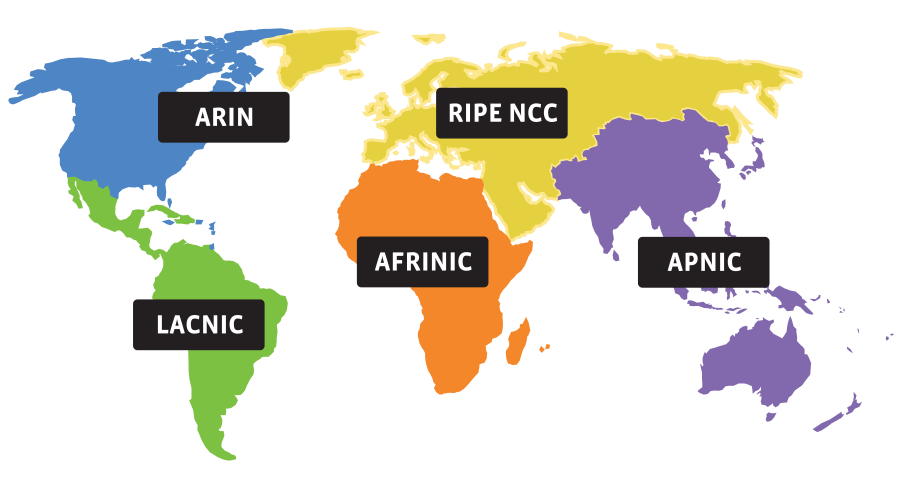
\includegraphics[scale=1.5]{img/rir-map.png} \\
        {\small Fonte: IANA (2020).} 
    \end{figure}
    
%\subsection{Cálculos VLSM}

    Um endereço IPv4 é um número de 32 bits, sendo representado na forma \textit{a.b.c.d/x}, em que \textit{x} é um número inteiro entre 0 e 32 que indica o tamanho do prefixo da rede, o qual representa a quantidade de bits da máscara da rede. Por exemplo, uma máscara 255.255.255.0 é representada por /24. Os $(32 - x)$ bits restantes são os bits dos \textit{hosts}. Essa representação é denominada CIDR (Classless Inter-Domain Routing), uma representação sem classes, adotada após o endereçamento com classes (A, B, C, D e E) cair em desuso devido ao desperdício na alocação de endereços.
    
    Cálculos de VLSM (Variable Length Subnet Masking) operam sobre o CIDR e permitem a criação de sub-redes dentro de uma sub-rede (recursivamente). Por exemplo, um ISP tem uma rede /21 alocada pelo NIC.br e pode dividi-la em sua intranet em 8 sub-redes /24, ou em 4 sub-redes /23 ou até mesmo em 2 sub-redes /23 mais 4 sub-redes /24 de maneira mista.

\subsection{Mitigando a escassez do IPv4 com CGNAT}

    O número de dispositivos conectados à internet tem crescido de tal forma que ultrapassou a capacidade de atendimento de IPs que um ISP pode oferecer aos seus assinantes. Para contrornar isso, a estratégia adotada é, a princípio, oferecer um IP público na interface de saída do roteador de borda (WAN) da sub-rede do cliente e uma faixa de endereços privados na rede local (LAN) do mesmo, sendo feita a tradução de endereços na interface WAN/LAN. IPs privados são blocos definidos pela RFC 1918 e que não devem ser anunciados na internet, sendo restritos ao uso em intranets para o funcionamento do artifício do NAT (network address translation).
    
    Existem ISPs que não possuem endereços o suficiente para todos os assinantes, sendo necessário recorrer ao recurso do CGNAT (Carrier-grade NAT) para contornar o problema. O CGNAT implementa uma camada de NAT na WAN do cliente, deixando de entregar um IP público para alocar um IP privado ao gateway cliente. IPs privados de CGNAT são definidos pela RFC 6598 e é através deles que é implantado o NAT da operadora, em que um mesmo endereço público é compartilhado por vários assinantes.

% \subsection{Motivação para o uso de NAT}
   
   O NAT funciona porque é a camada de transporte a responsável em estabelecer comunicação entre dois hosts e não a camada de rede, isto é, uma porta definida pelos respectivos sistemas operacionais dos hosts garante a conexão fim-a-fim na internet. Assim, a função do IP é rotear os pacotes e do TCP estabelecer a conexão HTTP, por exemplo. Um cliente com IP público dedicado tem a sua disposição 65535 portas, o que lhe daria a possibilidade de estabelecer, teoricamente ao máximo, 65535 conexões simultâneas.
   
   Como no NAT os clientes finais compartilham um único IP público, todas as portas que estão associadas a esse IP serão distribuídas entre eles pelo roteador de NAT, sendo que para cada solicitação de conexão será inserido na tabela de tradução de endereços o par $ ( IP_{publico}, \; Porta_{publica} ) $ associado com o par $ ( IP_{privado}, \; Porta_{privada} ) $ de forma aleatória e não conflituosa caso o par já exista na tabela, dado um tempo de vida para esse vínculo. Essa técnica tradicional de NAT é conhecida como \textit{masquerade}, por mascarar toda rede privada atrás do NAT através de um único IP.
   
\subsection{Aspectos legais quanto ao uso de NAT}
\label{sec:marco_civil}

   Embora a técnica de NAT \textit{masquerade} resolva o problema da escassez de endereços públicos, existe uma particularidade que não pode ser omitida. De acordo com o Art. 13 do Marco Civil da Internet (Lei nº 12.965/2014), ``na provisão de conexão à internet, cabe ao administrador de sistema autônomo respectivo o dever de manter os registros de conexão [...] pelo prazo de 1 (um) ano'', sendo que um registro de conexão é definido pelo ``conjunto de informações referentes à data e hora de início e término de uma conexão à internet, sua duração e o endereço IP utilizado pelo terminal'' \cite{lei12965}. A lei ainda destaca no Art. 22 que um juiz pode ordenar ao ISP o fornecimento dos registros de conexão à internet de um determinado cliente com a finalidade de obtenção de provas para processos judiciais.
   
   Dessa forma, o ISP tem a obrigação legal de manter o rastreio sobre qual IP cada um de seus clientes utilizou para navegar na internet, pois caso ele esteja utilizando a rede para cometer algum crime, a polícia conseguirá encontrá-lo. Isso parte do princípio de que na internet todos devem ser identificados pelo IP como sendo seu endereço virtual, porém o NAT \textit{masquerade} quebra essa identidade por não ser determinístico na tradução do endereço. Por isso, um ISP não pode simplesmente resolver a escassez por IPs utilizando uma metodologia de NAT desenvolvida para redes de escritórios domésticos e de pequenas empresas. No ISP, deve ser utilizada, por questões legais, a técnica específica e determinística chamada de CGNAT, também conhecida como NAT de operadora.

\subsection{Técnicas de CGNAT}

    Existem duas técnicas adotadas na implantação do CGNAT determinístico: o CGNAT horizontal e o vertical. Ambas garantem a operação do NAT, sendo a diferença entre uma e outra simplesmente a metodologia utilizada no mapeamento entre as redes público-privadas e as faixas de porta.
    
    No modelo horizontal, o mapeamento entre os endereços públicos e privados é feito horizontalmente para uma faixa determinada de portas, como é ilustrado na Figura \ref{fig:cgnat_horizontal}, em que o sentido de crescimento numérico dos endereços privados acompanha os endereços públicos. Essa técnica possibilita a implantação simplificada por uso de ferramentas de \textit{netmapping}.
    
    \begin{figure}[!htb]
        \centering
        \caption{Ilustração do modelo de CGNAT horizontal.} 
        \label{fig:cgnat_horizontal} 
        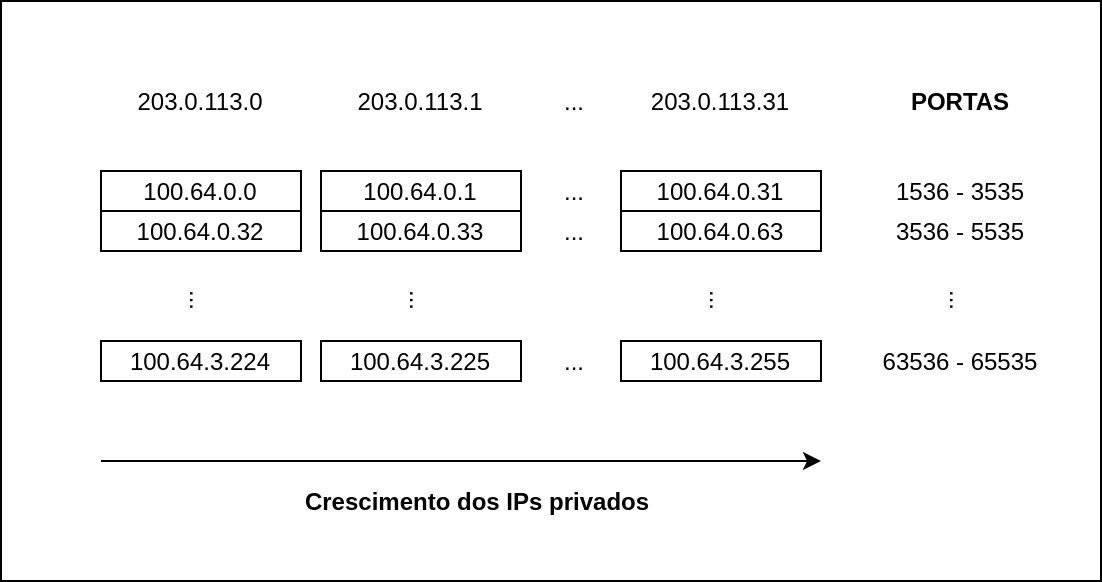
\includegraphics[width=0.9\linewidth]{img/CGNAT-Horizontal.png} \\
        {\small Fonte: do autor (2020).} 
    \end{figure}
    
    No modelo vertical, o sentido de crescimento dos IPs privados não coincide com os IPs públicos, pois o sentido desta vez segue o crescimento do range de portas. Assim, é tomado um IP público como referência e são mapeadas as faixas de portas para os IPs privados consecutivamente, como pode ser visto na Figura \ref{fig:cgnat_vertical}. Essa técnica é de mais fácil entendimento, porém requer mais trabalho para implantação por demandar criação de várias regras individuais de NAT.
    
    \begin{figure}[!htb]
        \centering
        \caption{Ilustração do modelo de CGNAT vertical.} 
        \label{fig:cgnat_vertical} 
        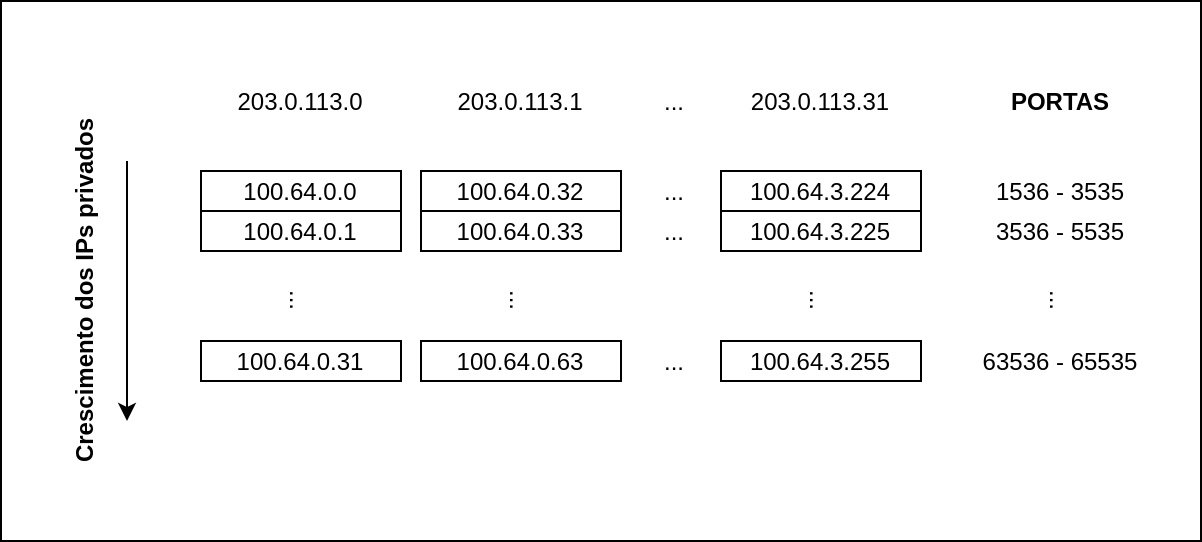
\includegraphics[width=0.9\linewidth]{img/CGNAT-Vertical.png} \\
        {\small Fonte: do autor (2020).} 
    \end{figure}

\subsection{Desvantagens do NAT}

    Apesar de solucionar a escassez de endereços de um ISP, o CGNAT implementa uma camada dupla de NAT para os assinantes, o que não permite o funcionamento de redirecionamentos de portas de maneira simples e direta. O redirecionamento de portas nesse cenário, necessita da compatibilidade do dispositivo adotado para implantação do CGNAT e fica limitado a uma faixa de portas definida pelo mapeamento.
    
    Como consequência do NAT duplo, protocolos P2P não funcionam, pois não existe comunicação de entrada direta com o \textit{host}, sendo necessário o uso de recursos para travessia de NAT, como reversão de conexão ou repasses para aplicação com um nó intermediário para resolução da limitação imposta \cite{kurose2014}.
    
    Do ponto de vista do modelo OSI, o NAT viola o encapsulamento da pilha de protocolos por trabalhar em conjunto nas camadas de rede e de transporte, com a tradução entre IP e porta, sem hierarquia. 
    
\subsection{Migração para IPv6}
    
    Como solução aos problemas estruturais e operacionais do NAT, foi proposta a migração para o IPv6 (IP versão 6), que adota como endereço um número de 128 bits, muito mais do que o suficiente para endereçar unicamente todos os dispositivos em LAN sem o uso de IPs privados. Como todos os dispositivos podem ter um IP público através do IPv6, não é necessário o conceito de NAT com o novo protocolo.
    
    Embora o IPv6 seja a solução, não basta apenas o ISP implantá-lo, é necessário que o acordo de tráfego no novo protocolo também esteja fechado com os servidores de sistemas e de provedores de conteúdo. Enquanto isso não for um tecnologia de ponta-a-ponta, o CGNAT é um modelo satisfatório no processo de transição.

\section{Segurança de ambientes de rede}

    Sistemas em rede estão suscetíveis a ataques, pois a internet é promíscua por sua própria natureza. O objetivo da segurança é minimizar os riscos, pois não existe sistema 100\% seguro. A cada dia são descobertas novas falhas e as correções também evoluem de forma constante.
    
    A segurança da informação é regida por quatro pilares: autenticidade, confidencialidade, integridade e disponibilidade. A segurança de redes tem seu foco principal em disponibilidade, prezando pela minimização de vulnerabilidades que possam ser exploradas para causar interrupção no serviço, sejam exploradas através de falhas físicas ou através de ataques de negação de serviço.
    
    Entre as principais ferramentas de defesa disponíveis para segurança de rede, estão o firewall e a VPN (Virtual Private Network), que serão descritas a seguir.

\subsection{Firewall}

    Firewall é um ponto entre duas ou mais redes onde é possível controlar todo o tráfego de dados que passa através dele. Assim, esse ponto único constitui um mecanismo utilizado para proteger uma rede confiável de uma rede pública não-confiável \cite{nakamura2007}.
    
    As técnicas básicas de firewall são a filtragem de pacotes estática (\textit{stateless}) e a filtragem de pacotes baseada em estados (\textit{stateful}). No firewall \textit{stateless}, as regras são aplicadas na camada de rede (camada 3) e de transporte (camada 4), sendo feita a filtragem a partir das informações de IP, porta e protocolo contidas no cabeçalho do pacote. A técnica \textit{stateless} apresenta alto desempenho e performance para gerenciamento de tráfego devido a sua simplicidade. Em contrapartida, não é uma técnica suficiente para filtragem de serviços de portas dinâmicas, em que as portas de comunicação são definidas em tempo de execução, como nos protocolos RPC e FTP \cite{nakamura2007}. O problema das portas dinâmicas é possível de ser tratado com um firewall \textit{stateful}, que mantém registros das conexões para filtragens mais inteligentes e dinâmicas, tendo como custo um maior consumo de recursos de processamento.
    
    As vulnerabilidade de obtenção de informação, em que atacantes oportunistas podem conseguir informações em banners de protocolos de rede local expostos na internet, podendo conseguir informações valiosas para auxiliar em um ataque de invasão, podem ser tratadas com firewall pelo uso de regras de acesso definidas por IP. Além disso, a vulnerabilidade de invasão também pode ser corrigida com um firewall fazendo bloqueio de portas aos invasores. 

    O bloqueio de portas também auxilia na minimização de ataques de negação de serviço, pois um atacante pode conseguir amplificar o tráfego e congestionar a rede explorando protocolos como DNS e SSDP, que têm o pacote de resposta muito maior que a requisição, podendo inundar a rede em um ataque coordenado. Com as portas desses serviços fechadas àqueles que não necessitam acessá-las, mais segurança é agregada à rede.
    
    O firewall não é a solução total para segurança da rede. É fundamental selecionar os usuários que podem acessar a rede e definir os seus respectivos níveis de acesso (somente leitura ou leitura e escrita). A autenticação e a autorização são também importantes aspectos a serem implementados na infraestrutura de segurança \cite{nakamura2007}.

\subsection{VPN}

    Uma VPN tem como funcionalidade prover conexão a uma rede local através da internet por meio de um túnel de conexão criptografado. O mecanismo da VPN provê serviço de acesso remoto como também serve de mecanismo para controle de acesso, fornecendo uma camada de autenticação à rede interna e de autorização quando combinada com um firewall.
    
    Os conceitos que fundamentam a VPN são a criptografia e o tunelamento. A criptografia é utilizada para garantir a autenticidade, o sigilo e a integridade dos dados através da conexão, e é a base da segurança dos túneis VPN \cite{nakamura2007}. Uma VPN implantada com protocolo PPTP ou L2TP garante somente autenticidade, enquanto IPSec e protocolos baseados em TLS (como Stunnel e aplicações modernas de VPN) somam integridade e confidencialidade ao túnel.

\section{Topologia de um ISP}

    O modelo comum de topologia adotado por operadoras de internet é formado por um triângulo entre roteadores B-RAS (\textit{broadband remote access server}), CGNAT e borda, conforme Figura \ref{fig:isp}. Os clientes finais conectam-se à rede através de PPPoE ao roteador B-RAS, que por sua vez encaminha o tráfego de IP público à borda que será roteada para a internet. Tráfego de IP privado de CGNAT (RFC 6598) é encaminhado ao equipamento que traduz os IPs privados em públicos antes de serem roteados à internet pela borda.
    
    Dependendo da dimensão da rede, é possível adotar modelos simplificados para economia de recursos, fazendo a mescla das funções de um ou de mais equipamentos em um único, desde que o equipamento suporte essa configuração.
    
    A Figura \ref{fig:isp} é uma representação genérica de camada 3 do núcleo da rede de um ISP. Existem muitos outros elementos de conexão de camada 2 e de camada 1 (lógica e física respectivamente) entre os dispositivos que não estão na imagem, como enlaces de rádio ou de fibra óptica. Também foi omitido, por simplificação, que dentro do salto entre o ABR e a Internet na Figura \ref{fig:isp}, existe o ASBR (Autonomous System Border Router), que é resposável por rotear o tráfego para a internet.
    
    \begin{figure}[!htb]
        \centering
        \caption{Modelo de topologia de um ISP.} 
        \label{fig:isp} 
        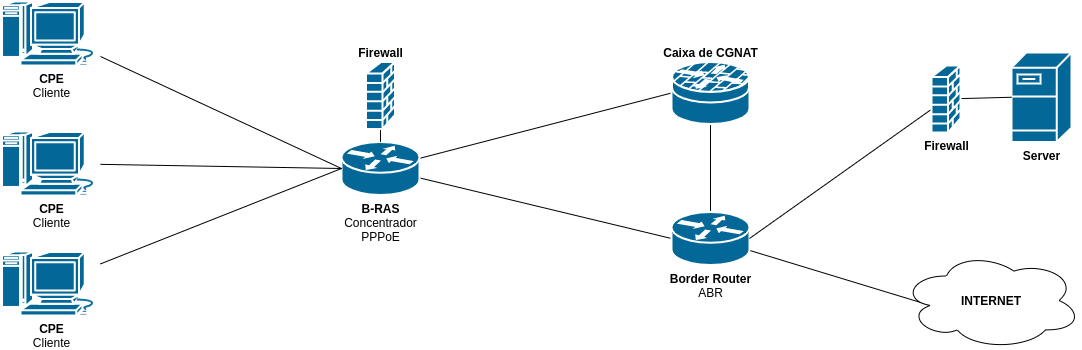
\includegraphics[width=0.9\linewidth]{img/isp.png} \\
        {\small Fonte: do autor (2020).} 
    \end{figure}
    
    Na infraestrutura lógica do ISP, também entram os servidores de serviços locais, que provêm servidores de autenticação RADIUS, serviço de DNS local para respostas mais rápidas, Proxy HTTP\footnote{Também conhecido como CDN -- content distribution network.} para poupar consumo de banda de acesso à internet e serviço de VPN.
    